\chapter{Experimental Result}
\label{chapter:Experimental_Result}

\section{Experiment environment}

\subsection{OS used for the experiment}

\begin{tabular}{lll}
Distributor ID: & Ubuntu &             \\ 
Description:    & Ubuntu & 18.04.4 LTS \\
Release:        & 18.04  &             \\
Codename:       & bionic &             \\
\end{tabular} 


\subsection{CPU used for the experiment}

\subsubsection{Specification of CPU1}

\begin{tabular}{ll}
product:     & AMD Ryzen 7 3700X 8-Core Processor \\
vendor:      & Advanced Micro Devices [AMD] \\
bus info:    & cpu@0 \\
size:        & 3035MHz \\
capacity:    & 3600MHz \\
width:       & 64 bits \\
threads:     & 16 \\
\end{tabular} 

\subsubsection{Specification of CPU2}

\begin{tabular}{ll}
product:     & AMD Ryzen Threadripper 2920X 12-Core Processor \\
vendor:      & Advanced Micro Devices [AMD] \\
bus info:    & cpu@0 \\
size:        & 3291MHz \\
capacity:    & 3500MHz \\
width:       & 64 bits \\
threads:     & 24 \\
\end{tabular} 


\section{Experimental conditions}

\begin{comment}
NGSIM車両走行データに含まれている、US101およびI80の路上を走行する45分間の車両のデータを使用した。
観測は10Hzで、1秒に10個のサンプルポイントが存在する。
渋滞前の状態と、渋滞中の状態が両方含まれている。

全部の車両データの中から、ランダムに1個のトラジェクトリを選択し、その車両を学習済みポリシによる自動運転車両と交換して、オリジナルの車両との間の差異を計算する。
ポリシは確率ポリシであるため、軌道一つに対して20回のトライアルを行う。
トラジェクトリの選択は全部で1000回行われた。

エゴ車両ではない周辺車両は、NGSIMの走行トラジェクトリをそのまま走行する。エゴ車両が接近しても進路を変更することはないが、ブレーキを行うことはある。
\end{comment}

We used the data for 45 minutes of vehicles running on US 101 and I80 roads, which was included in the {\it NGSIM} vehicle driving data.
The observation is 10 Hz, and there are 10 sample points per second.
Both the state before traffic jam and the state during traffic jam are included.


One trajectory is randomly selected from all the vehicle data, and the vehicle is replaced with an autonomous vehicle according to the learned policy, and the difference between the original vehicle and the original vehicle is calculated.
Since the policy is a probabilistic policy, 20 trials are performed for each orbit.
A total of 1000 trajectory selections were made.

Peripheral vehicles that are not ego vehicles will continue to run on the {\it NGSIM} travel trajectory. It does not change course when an ego vehicle approaches, but it may brake.


\subsection{Metrics}


This section details the metrics for vehicle behavior that are evaluated by the validation program.

Speed, acceleration and jerk are calculated from the sample point to be calculated and the sample point one previous point (0.1 second before).
Speed is calculated from the position of the sample point and the position of the previous sample point, acceleration is calculated from the speed of the sample point and the speed of previous sample point, jerk is calculated from the acceleration of the sample point and the acceleration of the previous sample point.
Future sample points are not used.

\begin{comment}
速度、加速度、jerk は、計算を行うサンプル点とそのひとつ前(0.1秒前のサンプル点)から計算する。
速度は、サンプル点と一つ前のサンプル点の位置から計算され、加速度は、サンプル点と一つ前のサンプル点の速度から計算され、jerkは、サンプル点と一つ前のサンプル点の加速度から計算される。
未来のサンプル点は使用されていない。

サンプルは1秒に10回(つまり10Hz)行われ、トラジェクトリは10秒間である。一つのトラジェクトリは100のサンプルポイントからなる。
\end{comment}

The sample is taken 10 times per second (ie 10Hz) and the trajectory is 10 seconds. Therefore, one trajectory consists of 100 sample points.
The following metrics are calculated on that basis.

\subsubsection{Root Weighted Square Error.}

The square of the two-dimensional distance, lateral distance, and speed difference between the expert vehicle and the learning vehicle. The smaller value means learning policy is more similar to the expert.

\begin{tabular}{ll}
Position & 2 dimensional distance.  \\
Lane Offset & Lateral distance from lane center. \\
Speed & Longitudinal speed of vehicle heading direction. \\
\end{tabular}


\subsubsection{Kullback-Leibler Divergence}

The KL divergence of the probability distributions of the expert policy $\pi_E$ and the reinforcement learning policy $\pi_\theta$ is shown. The smaller  value means the learning policy is more similar to the expert.

\begin{tabular}{ll}
iTTC  & Inverse time to collision. \\
Speed & Longitudinal speed of vehicle heading direction. \\
Acceleration & Longitudinal acceleration of vehicle heading direction. \\
Turn-Rate & Turn-rate of vehicle heading. \\
Jerk & Longitudinal jerk of vehicle heading direction. \\
\end{tabular}


\subsubsection{Emergent Value}

It is a metric for unfavorable driving, such as emergency braking or running off the track. The smaller values means driving is safety.
In the following metrics, 1 represents once.
There are 100 sample points on the trajectory, 
offroad duration is 100.0 if all the trajectories are off the track.
Only collision is calculated so that the maximum value of one trajectory is 1.

All the calculation methods follow the original paper.\cite{DBLP:journals/corr/KueflerMWK17}


\begin{tabular}{ll}
Lane Change Rate & It is the number of lane changes made in 10 seconds. \\
Offroad Duration & It is the number of spent off road in 10 seconds. \\
Collision Rate   & It is the number of collision made in 10 seconds. \\
Hard Break Rate  & It is the number of spent hard break in 10 seconds. \\
\end{tabular}


\section{Description of this result}

In this section, {\tt MLP-AUT}, {\tt GRU-AUT} are learned data by Author, and {\tt MLP}, {\tt GRU} are learned data by this experiment.


Author's data includes 500 iterations in MLP and GRU. The authors' programs used 447 iterations in the MLP and 413 iterations in the GRU without explanation, so they are shown here.

In this experiment, iteration 499 of generated leaned data are used.




\section{Root Weighted Square Error}


\begin{figure}[H]
\begin{center}
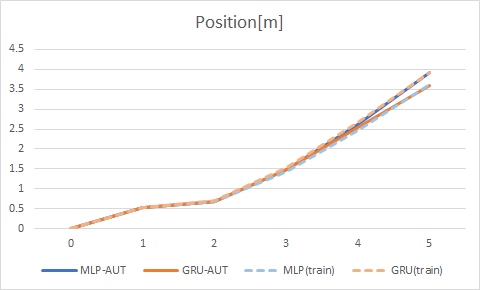
\includegraphics[width=14cm]{./figures/graph_position.png}
\caption{Speed Error Comparison}
\label{fig:graph_position}
\end{center}
\end{figure}

\begin{figure}[H]
\begin{center}
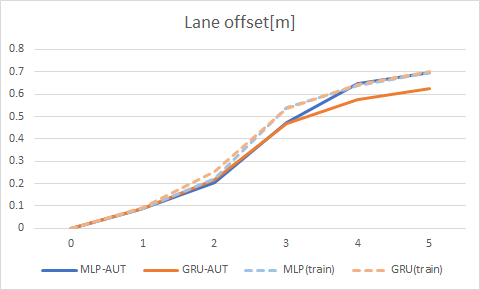
\includegraphics[width=14cm]{./figures/graph_lane.png}
\caption{Speed Error Comparison}
\label{fig:graph_lane}
\end{center}
\end{figure}

\begin{figure}[H]
\begin{center}
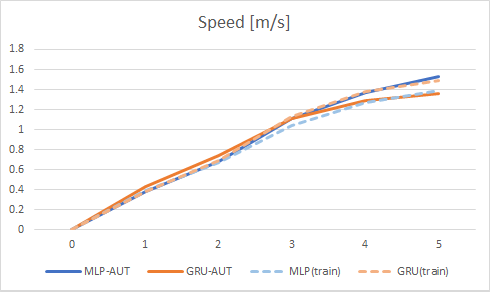
\includegraphics[width=14cm]{./figures/graph_speed.png}
\caption{Speed Error Comparison}
\label{fig:graph_speed}
\end{center}
\end{figure}


\section{Kullback-Leibler Divergence}


\begin{figure}[H]
\begin{center}
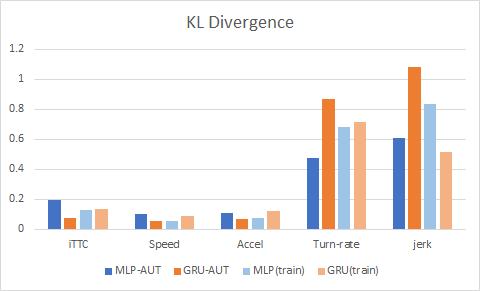
\includegraphics[width=14cm]{./figures/graph_kldivergence.png}
\caption{KL Divergence}
\label{fig:graph_kldivergence}
\end{center}
\end{figure}


\section{Emergent Value}

\begin{figure}[H]
\begin{center}
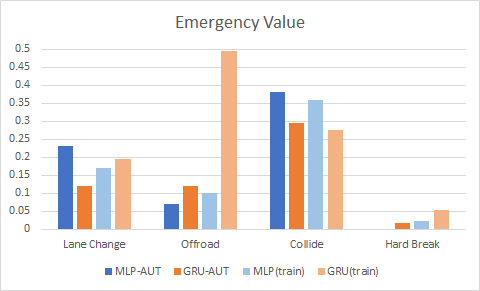
\includegraphics[width=14cm]{./figures/graph_emergency.png}
\caption{Emergent Value}
\label{fig:graph_emergency}
\end{center}
\end{figure}
